\begin{frame}
    \frametitle{Particle Filter}
    \note{Information taken from Cyrill Stachniss's video https://youtu.be/MsYlueVDLI0}
    \footnotesize
    \begin{itemize}
        \item With EKF, we are restricted to Gaussian distributions.
        \item When we use EKF, we obtain a Gaussian distribution that describes where the robot is located.
        \item In Particle Filter, we use particles or hypotheses that describe where the robot could be.
        \item Instead of having a parametric form like EKF, which describes the probability distribution with the parameters mean $\mu$ and covariance $\covariance$, Partible Filter uses non-parametric samples as hypotheses about where the robot could be.
        
    \end{itemize}
    
    \begin{center}
        \movie[loop]{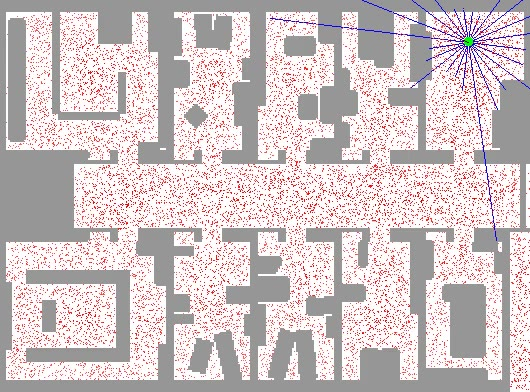
\includegraphics[width=0.4\columnwidth]{images/particle_filter/particle_filter_video.jpg}}{videos/particle_filter.mp4}
    \end{center}
    
    \note{Video taken from https://rse-lab.cs.washington.edu/projects/mcl/animations/global-floor.gif}
    
\end{frame}
    
\begin{frame}
    \frametitle{Flexible Function Approximation}
    \note{Information taken from Cyrill Stachniss's video https://youtu.be/MsYlueVDLI0}
    \footnotesize
    
    \begin{itemize}
        \item Goal: To be able to estimate any \textbf{arbitrary probability distribution}.
    \end{itemize}
    
    \begin{center}
        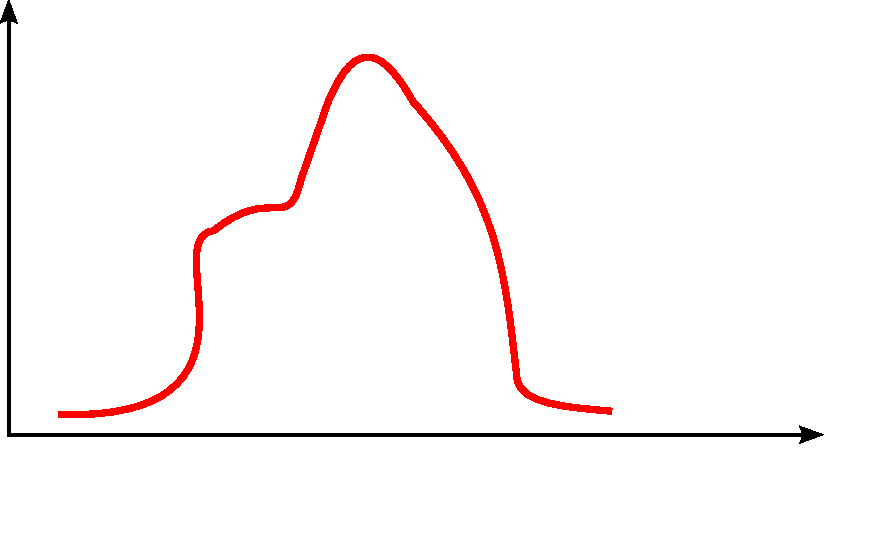
\includegraphics[width=0.5\columnwidth]{./images/particle_filter/arbitrary_distribution.pdf}
    \end{center}
    
\end{frame}
    
\begin{frame}
    \frametitle{Using Samples (Particles)}
    \note{Information taken from Cyrill Stachniss's video https://youtu.be/MsYlueVDLI0}
    \footnotesize
    \begin{itemize}
        \item \textbf{Multiple samples} to represent an arbitrary probability distribution
        \item Samples are more clustered in some areas and less so in others. The number of particles per unit area describes how likely it is that the robot is in that area.
        \item Each sample accumulates a bit of ``probability mass''
        \item Samples can be viewed as an approximation to the probability density function (pdf).
        \item To obtain the PDF, you must integrate over a certain area to obtain the mathematical probability that the robot is in that area.
    \end{itemize}
    
    \begin{center}
        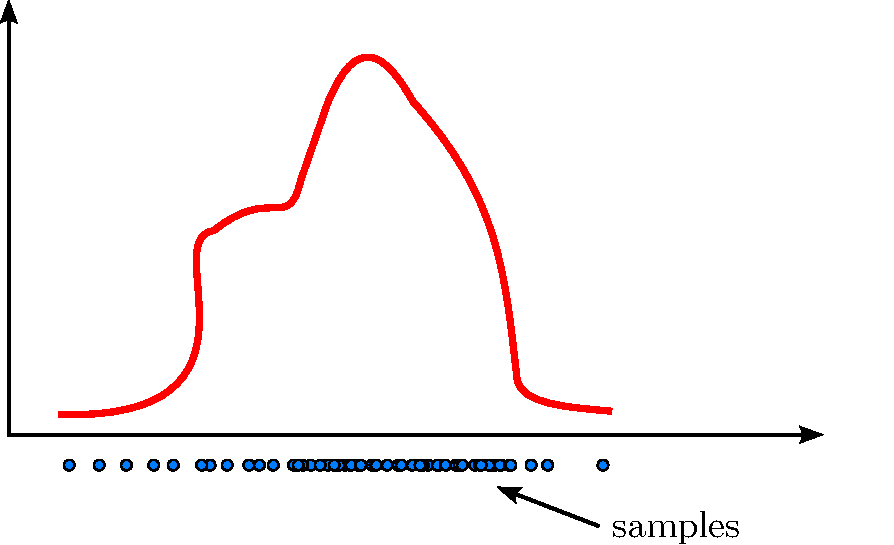
\includegraphics[width=0.5\columnwidth]{./images/particle_filter/arbitrary_distribution_samples.pdf}
    \end{center}
    
\end{frame}
    
\begin{frame}
    \frametitle{Using Weighted Samples}
    \note{Information taken from Cyrill Stachniss's video https://youtu.be/MsYlueVDLI0}
    \footnotesize
    \begin{itemize}
        \item \textbf{Multiple Weighted Samples} to Represent an Arbitrary Probability Distribution
        \item We can reduce the number of samples we need by adding weights to each sample.
        \item The more weight a sample has, the more probability mass there is in that region.
        \item The weights of all the particles together must sum to 1.
        \item Initially, we could add a uniform weight to each sample. For example, if we have $n$ samples, then each sample has weight $\frac{1}{n}$
    \end{itemize}

    \begin{center}
        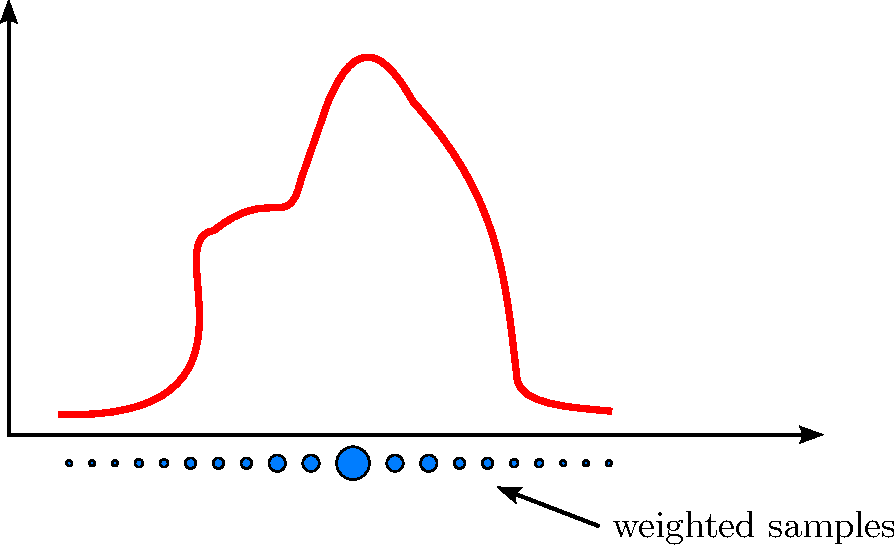
\includegraphics[width=0.5\columnwidth]{./images/particle_filter/arbitrary_distribution_weighted_samples.pdf}
    \end{center}

\end{frame}
    
\begin{frame}
    \frametitle{Particle Filter}
    \note{Information taken from Cyrill Stachniss's video https://youtu.be/MsYlueVDLI0}
    
    \footnotesize
    \begin{itemize}
        \item Note that this is an approximation of the pdf.
        \item It is important to have a sufficient number of samples to adequately represent the pdf.
    \end{itemize}

\end{frame}
    
    
\begin{frame}
    \frametitle{Material for Particle Filter}

    \begin{itemize}
        \item Information extracted from Video by Cyrill Stachniss https://youtu.be/MsYlueVDLI0
        \item https://rse-lab.cs.washington.edu/projects/mcl/
    \end{itemize}

\end{frame}


\begin{frame}
    \frametitle{TODO}
    \note{Information taken from Cyrill Stachniss Video https://youtu.be/MsYlueVDLI0}
    \note{https://rse-lab.cs.washington.edu/projects/mcl/}

    \TODO{USE THE SEMINAR SLIDE}

\end{frame}